\section{Оборудование}
Схема для исследования гальванометра в стационарном режиме. Постоянное напряжение снимается с блока
питания и измеряется вольтметром. Ключ позволяет менять направление тока через гальванометр,
делитель напряжения~--- менять величину тока в широких пределах. Ключ служит для включения
гальванометра, кнопка~--- для его успокоения. Магазин сопротивлений позволяет менять режим работы гальванометра от колебательного до апериодического.

При $R_{1} \ll R,\;R_{0},\;R_{2}$ сила тока, протекающего через гальванометр, может быть вычислена как 
\[
    I = \frac{R_{1}}{R_{2}}\frac{U_{0}}{R+R_{0}}
\]
$U_{0}$~--- показания вольтметра, $R_{1}/R_{2}$~--- положение делителя, $R$~--- сопротивление магазина, $R_{0}$~--- внутреннее сопротивление гальванометра.

Угол отклонения рамки от положения равновесия измеряется с помощью осветителя, зеркальца, укреплённого на рамке, и шкалы, на которую отбрасывается луч света от зеркальца. Координата $x$ светового
пятна на шкале связана с углом $\varphi$ отклонения рамки формулой
\[
    x = a\arctg 2\varphi
\]
\[
    C_{I} = 2aI/x
\]

Критическим сопротивлением баллистического гальванометра называется сопротивление его электрической цепи $R_{\text{кр}}$,  при котором после начального толчка подвижная система почти экспоненциально возвращается к нулю. На практике критический режим, требующий строгого выполнения условия не может быть
точно реализован и имеет значение как пограничный между режимом
затухающих колебаний  и режимом апериодического затухания.

\begin{figure}[ht!]
    \center{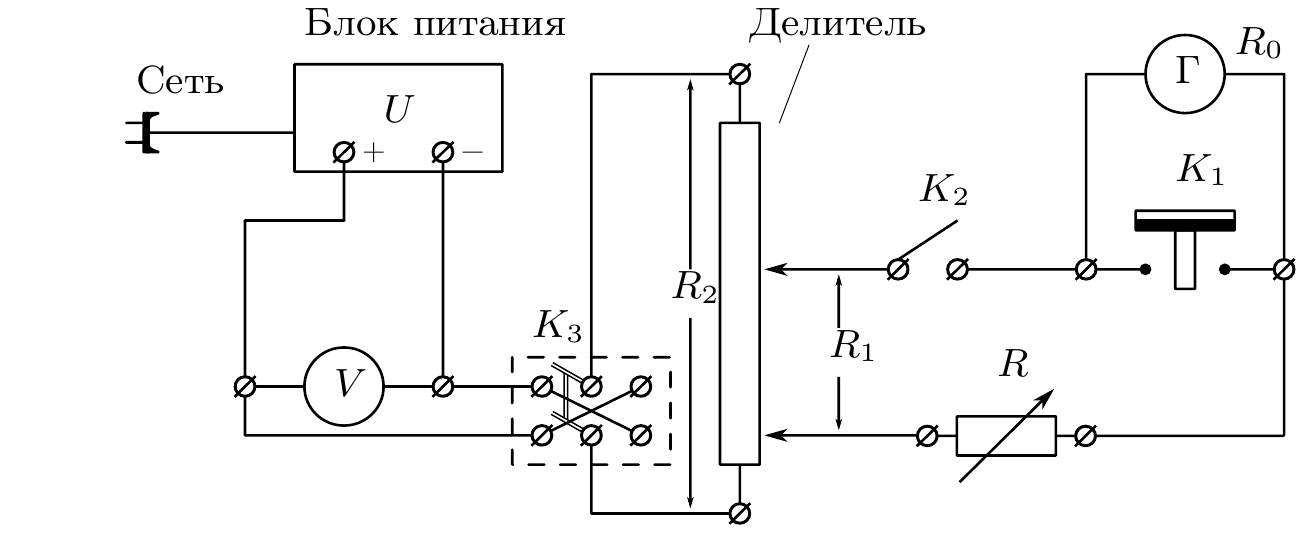
\includegraphics[width=0.8\linewidth]{../img/eq1.png}}
\end{figure}

\[
    \Theta = \gamma T_{1} = \ln\frac{x_{n}}{x_{n+1}}
\]
\[
    \sqrt{\frac{4\pi^{2}}{\Theta}+1} = \frac{R+R_{0}}{R_{\text{кр}}+R_{0}}
\]

Для изучения работы гальванометра в режиме измерения заряда (вбаллистическом режиме), используется схема.

\begin{figure}[ht!]
    \center{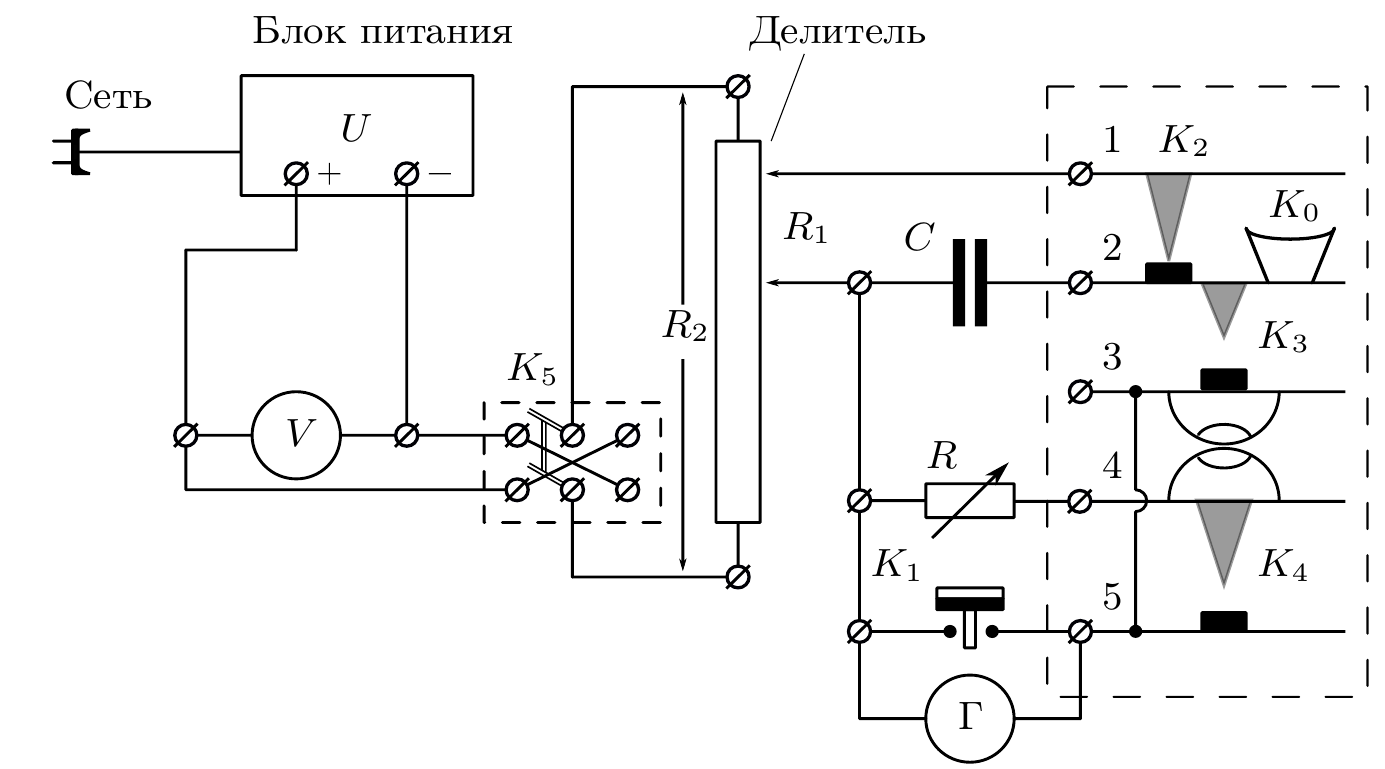
\includegraphics[width=0.8\linewidth]{../img/eq2.png}}
\end{figure}
\[
    \varphi_{max}^{\text{св}} = \varphi_{0}\left(1+\frac{\Theta}{4}\right)
\]
\[
    C_{q} = 2a\frac{R_{1}}{R_{2}}\frac{CU_{0}}{x_{max}}
\]

